In assembly, computation, and readout of single atoms, laser cooling and trapping techniques play a central role. This chapter will give some background on how this technique works, and how we intend to apply it onto strontium (Sr).

\section{Magneto-Optical Trap}

The workhorse for producing clouds of ultracold atoms is the 3D \ac{MOT}. In essence, it consists of three sets of counter-propagating beams as well as a magnetic field gradient, together providing a dampening as well as a confining force. 

\subsection{Doppler Cooling}

Consider an atom with ground state $\ket{g}$ and excited state $\ket{e}$ separated by energy splitting $\hbar \omega_0$. This convention will be used for the remainder of this work. We drive a laser with omega $\omega$ that is near-resonant, but \emph{detuned} slightly from the transition by an amount $\delta$:

\begin{equation}\label{detuning}
	\delta = \omega - \omega_0
\end{equation}

It will turn out that detuning is one of the most important parameters in laser cooling. In this work we will always have $\delta <0$. Because of the Doppler effect, the atom 'sees' a slightly different light frequency depending on its velocity $v$ according to $\delta'=\delta+kv$ and the laser may become resonant: $\delta' = \omega_0$, causing the atom to absorb a photon absorbing momentum $\hbar k$ and promoting an electron to the excited state $\ket{e}$. When spontaneous emission causes the atom to fall back in a time $\tau = 1/\gamma$ where $\gamma$ is the linewidth of the transition, the electron is decayed back to the ground state, but the emitted photon is emitted in a random direction. This can be repeated many times per second at a scattering rate $\Gamma_{\text{sc}}$ \cite{Metcalf1999}

\begin{equation}\label{eq:ScatteringFrequency}
	\Gamma_{\text{sc}} = \frac{ \gamma s_0 /2}{1+s_0+\left[2(\delta+ k v)/\gamma\right]^2},
\end{equation}

where $s_0 = I/I_{sat}$ is the saturation parameter as a function of the light intensity $I$ for saturation intensity $I_{sat} = \hbar c \gamma \pi/3\lambdaup^3$ for wavelength $\lambda$ and linewidth $\gamma$. Because the absorption occurs in a fixed direction and the emission is a random event, the atom will experience a net force scattering force $F = \hbar k \Gamma_{sc}$.

\subsection{Optical Molasses}

We can reflect the laser beam using a mirror, such that the force works in both directions of the spatial coordinate. We will only consider one spatial coordinate which we will denote as $z$, but the treatment can be easily extended to 3 dimensions. The total force from both contributions from \cref{eq:ScatteringFrequency} is \cite{Kowalski2010}

\begin{equation}\label{eq:OpticalMolasses}
	F = \frac{\hbar k \gamma s_0}{2}\left\{\
	\left[1 + s_0 + 4\frac{(\delta+kv)^2}{\gamma^2}\right]^{-1}+
	\left[1 + s_0 + 4\frac{(\delta-kv)^2}{\gamma^2}\right]^{-1}
	\right\}
\end{equation}

We have plotted the result of \cref{eq:OpticalMolasses} in \cref{fig:MOTcooling} as a function of velocity in units of $\hbar / k$, such that it is dimensionless. Contributions of both beams, as well as their total force, are shown in units of $\hbar k \gamma$. Doing a series expansion to first order around $v = 0$. For $\delta<0$ we find we can linearize the force $F$ as \cite{Metcalf1999}

\begin{figure}
\centering
	\begin{subfigure}{.38\textwidth}
		\centering
		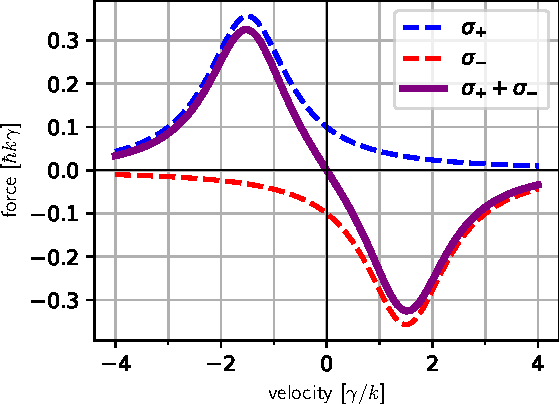
\includegraphics[width=\linewidth]{figures/MOTplot.pdf}
		\caption{}
		\label{fig:MOTcooling}
	\end{subfigure}
	\begin{subfigure}{.52\textwidth}
		\centering
		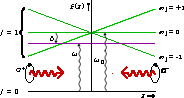
\includegraphics[width=\linewidth]{figures/OpticalMolasses.pdf}
		\caption{}
		\label{fig:MOTconcept}
	\end{subfigure}
	\caption{a) Cooling force from a magneto-optical trap. Contributions from the $F^+$, $F^-$ and the total force are shown for $\delta = -\gamma$ and $I/I_0 = 2.$ Concept of optical molasses in 1D. Atomic frequency is detuned from the atomic transition by $\delta<0$. Because of the linear magnetic field, for $z>0$, the $m_j=-1$ atoms become resonant with only $\sigma^+$ light because of selection rules, and vice versa.}
	\label{fig:MOTPlots}
\end{figure}

\begin{equation}\label{eq:ForceLinearized}
	F \sim - \hbar k^2 s_0 \frac{-2\delta/\gamma}{\left[1+s_0+(2\delta/\gamma)^2\right]^2} \equiv -\beta v
\end{equation}

Where $\beta$ is the slope of the scattering force around $v=0$. The resulting force has a dampening character on the velocity, which if applied in all 3 dimensions can cool atoms to ultracold temperatures. 

The treatment so far would suggest that this can be used to cool atoms to temperatures of absolute zero. This is not the case, as the random character of the scattering force means the atom fluctuates around the equilibrium velocity according to a Brownian motion. For $\delta=-\gamma/2$, \cref{eq:ForceLinearized} ($\beta$) is at a maximum, yielding the lowest possible temperature achievable using Doppler cooling: the Doppler temperature $T_D$ \cite{Metcalf1999}

\begin{equation}\label{eq:DopplerTemperature}
	T_D = \frac{\hbar}{2k_b} \gamma.
\end{equation}

where $k_b$ is Boltzmann's constant. Apparently, this cooling limit is only dependent on the linewidth of the transition $\gamma$, apart from physical constants. This result will be used later in \cref{sec:Sr}.

\subsection{Magnetic Trapping}

Apart from cooling the atoms, we want to trap them at a specific location to increase the density of atoms. We can use the Zeeman effect for this, which tells us the atomic energy levels will be split an amount $\Delta E$ according to \cite{Griffiths2004}

\begin{equation}\label{eq:Zeeman}
	\Delta E = \mu_{\emph{B}} g_J m_j B,
\end{equation}

where $\mu_{\emph{B}}$ Bohr magneton, $g_J$ the Landé g-factor, $m_j$ is the magnetic quantum number and $B_{\text{ext}}$ the applied magnetic field. The magnetic field is tuned in such a way that it is linear in all 3 dimensions and zero at the center of the \ac{MOT} by using a set of magnetic field coils in an anti-Helmholtz configuration. Because of the Zeeman splitting, the chance of the atoms coming in resonance with the laser varies with the position from the origin according to \cite{Kowalski2010}

\begin{equation}\label{eq:DetuningFull}
	\delta' = \delta + k v - \frac{\mu'B}{\hbar}
\end{equation}

Where $\mu' = (g_e m_e-g_g m_g)\mu_B$ is the effective magnetic moment for the transition \cite{Kowalski2010}. To ensure that atoms only absorb momentum kicks in the right direction, the laser beams are circularly polarized: $\sigma^+$ from the left and $\sigma^-$ from the right. Because the sign of the Zeeman shift is dependent on the magnetic quantum number $m_j$, selection rules prescribe that atoms displayed by $z>0$ are only resonant with $\sigma^-$-light and vice versa. This is sketched in \cref{fig:MOTconcept}. Inserting \cref{eq:DetuningFull} in \cref{eq:OpticalMolasses} yields

\begin{equation}\label{eq:MOTfull}
	\frac{F}{\hbar k \gamma s_0} = \frac{1}{2}\left\{\
	\left[1 + s_0 + 4\frac{(\delta+kv+\mu'B/\hbar)^2}{\gamma^2}\right]^{-1}+
	\left[1 + s_0 + 4\frac{(\delta-kv-\mu'B/\hbar)^2}{\gamma^2}\right]^{-1}
	\right\}
\end{equation}

Expanding \cref{eq:MOTfull} around $(v,z) = (0,0)$, keeping only first order terms finally leaves us with \cite{Kowalski2010}

\begin{equation}\label{eq:ForceMOT}
	F_{\text{MOT}}(z,v) \approx -\beta v - \kappa z.
\end{equation}

Where $\beta$ is the same we found in \cref{eq:ForceLinearized} and $\kappa \equiv \mu' \beta /\hbar k \cdot \partial B/\partial z$. Apart from the dampening force, we now also have a restoring force. When applied in 3 dimensions this can be used to make clouds of ultracold atoms. 

\section{Optical Dipole Traps}\label{sec:OpticalDipoleTrap}

While magneto-optical traps are excellent for producing clouds of ultracold atoms, the constant photon scattering is unwanted during qubit operation. Therefore, after the atom cloud is cooled in the \ac{MOT}, it is typically loaded in another type of trap: the \ac{ODT}. An ODT uses far-off-resonant light. Though this means that the coupling and therefore the trapping is weaker, it has negligible scattering, which is important to maintain coherence of quantum states. We consider a radiation field $\mathbf{E}$. This field will induce a dipole moment $\mathbf{p}$ in the atom according to 
	
\begin{equation}\label{eq:DipoleMoment}
	\mathbf{p} = \alpha \mathbf{E}.
\end{equation}

Consequently, the dipole potential will interact with the electric field leading to and an interaction dipole potential $U_{\text{dip}}$ as a function of the position vector $\mathbf{r}$ \cite{Grimm2000}

\begin{equation}\label{eq:DipolePotential}
	U_{\text{dip}}(\mathbf{r}) = -\mathbf{p}\mathbf{E} = 
	-\frac{1}{2} \left\langle \mathbf{p}\mathbf{E} \right\rangle = \frac{\operatorname{Re}(\alpha)}{2\epsilon_0 c} I(\mathbf{r}),
\end{equation}

where the $\left\langle\right\rangle$ brackets denote the time average. We average over this radidly varying phase term, yielding a factor $1/2$. Furthermore we used $I(\mathbf{r}) = |\mathbf{E}(\mathbf{r})|^2/(2\epsilon_0 c)$ where $\epsilon_0$ is the electric constant. The dipole force thus scales with the in-phase part of the polarizability with the light field. An additional factor $1/2$ comes in because the dipole moment is induced and not permanent \cite{Grimm2000}. The gradient of \cref{eq:DipolePotential} gives rise to the dipole force:

\begin{equation}\label{eq:DipoleForce}
	\mathbf{F}_{\text{dip}}(\mathbf{r}) = - \frac{\operatorname{Re}(\alpha)}{2\epsilon_0c}\nabla I(\mathbf{r})
\end{equation}

The dipole force can be used to coherently trap our qubits. To maximize the dipole force \cref{eq:DipoleForce}, we have to maximize the gradient of the light intensity profile. This can be done by focussing the laser on the smallest possible spot. How we do this is explained in \cref{ch:tweezer}. The scattering rate from the ODT can be found by averaging over the derivative of the dipole moment with the electric field \cite{Grimm2000}

\begin{equation}\label{eq:ScatteringRate}
	\Gamma_{\text{sc}}(\mathbf{r}) = \frac{\left\langle \mathbf{p} \mathbf{E} \right\rangle}{\hbar \omega}
	 = \frac{\operatorname{Im}(\alpha)}{\hbar \epsilon_0 c} I(\mathbf{r}).
\end{equation}

\cref{eq:DipoleForce,eq:ScatteringRate} are general expressions for any potential. The fact that $\alpha(\omega)$ is complex means there is a phase delay between the electric field and the dipole response. The task that remains is finding the polarizability $\alpha(\omega)$. As a starting point, we will consider the electron as a (classical) damped harmonic oscillator, which is for Alkali species already fairly accurate \cite{Grimm2000}.

\subsection{Classical}

In the classical picture, we assume a classical light field, as well as a classical electron (harmonic oscillator). We can write down a general expression for the the light field propagating in the $z$-direction polarized in the $\bm{\hat{\epsilon}}$ direction perpendicular to it:

\begin{equation}\label{eq:ClassicalField}
	\mathbf{E}(z,t) = \mathbf{E}_0 \cos{(k z - \omega t)} 	\bm{\hat{\epsilon}}
\end{equation}
	 
The electron is modeled as a damped harmonic oscillator (Lorentz oscillator). Integrating the equation of motion for the electron, assuming a dipole moment $\mathbf{p} = e \mathbf{r}$ where $r$ is the position yields after equating to \cref{eq:DipoleMoment} for the polarizability \cite{Grimm2000}

\begin{equation}\label{eq:LorentzOscillator}
	\alpha(\omega)=6 \pi \epsilon_{0} c^{3} \frac{\Gamma / \omega_{0}^{2}}{\omega_{0}^{2}-\omega^{2}-\mathrm{i}\omega^3\Gamma/\omega_0^2}
\end{equation},

Where $\Gamma$ is the on-resonant damping rate in terms of the electron mass $m_e$. 

\begin{equation}\label{eq:ResonantDampingRate}
	\Gamma = \frac{e^2 \omega_0^2}{6\pi \epsilon_0 m_e c^3}
\end{equation}

Inserting \cref{eq:LorentzOscillator} in \cref{eq:DipolePotential,eq:ScatteringRate} yields, after assuming $\delta \ll \omega, \Gamma \ll \omega$

\begin{equation}\label{eq:DipoleClassicalResult} 
	U_{\text{dip}}(\mathbf{r}) = 
	\frac{3\pi c^2}{2\omega_0^3}\frac{\Gamma}{\delta} I(\mathbf{r}),
	\quad
	\Gamma_{\text{sc}}(\mathbf{r}) = 
	\frac{3\pi c^2}{2\hbar\omega_0^3}\left(\frac{\Gamma}{\delta}\right)^2 I(\mathbf{r})
\end{equation}

From \cref{eq:DipoleClassicalResult} the relation these two quantities is $\hbar \Gamma_{sc} =\Gamma U_{\text{dip}}/\delta$. Thus, to keep scattering events to a minimum a large detuning should be used. To still have sufficiently deep traps, high light intensities are used. 


\subsection{Semi-Classical}

In the semi-classical picture, we consider the same classical light field \cref{eq:ClassicalField}, but consider an atom with quantized energy levels. We will consider a two-level atom with eigenstates $\ket{g}$ (ground) with energy $\hbar \omega_g$ and $\ket{e}$ (excited) with $\hbar \omega_e$, see \cref{fig:2LevelAtom}. Then the atomic Hamiltonian in this basis reduces to \cite{Loudon2000}

\begin{figure}
	\centering
	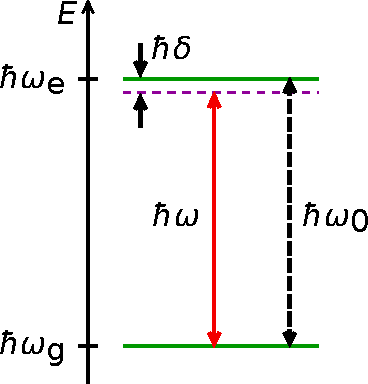
\includegraphics[height=4.1cm]{figures/2LevelAtom.pdf}
	\caption{Energy level scheme for the 2-level case. The two energies are split by $\omega_e - \omega_g = \omega_0$. The detuning is $\delta = \omega-\omega_0<0$ is shown as well.}
	\label{fig:2LevelAtom}
\end{figure}

\begin{equation}\label{eq:AtomHamiltonianMain}
	\mathcal{H}_A = \hbar \omega_g \ket{g}\bra{g} + \hbar \omega_e \ket{e}\bra{e}
\end{equation}

The radiation field is modeled as a time-dependent perturbation such that the total Hamiltonian is \cite{Leeuwen2017}

\begin{equation}\label{eq:PerturbationMain}
	\mathcal{H} = \mathcal{H}_A + \mathcal{H}_{I}(t),
\end{equation}

We can write down the combined wave function in the basis of the unperturbed eigenstates, its time evolution given by

\begin{equation}\label{eq:TwoLevelMain}
	\ket{\psi(t)} = c_g(t) e^{-i \omega_g t} \ket{g} + c_e(t) e^{-i \omega_e t} \ket{e}.
\end{equation}

In appendix \ref{ch:LightMatter} the Schrodinger equation is solved for the 2-level atom using the dipole approximation as well as the \acf*{RWA}. The following matrix equation is derived for the 2 level atom (\cref{fig:2LevelAtom}) \cite{Foot2005}

\begin{equation}\label{eq:MatrixEvolution}
	i \hbar \begin{pmatrix}
		\dot{c}_g \\ 
		\dot{c}e
	\end{pmatrix}
	= \frac{\hbar}{2} \begin{pmatrix}
		\delta & \Omega \\ \Omega^* & -\delta 
	\end{pmatrix} 
	\begin{pmatrix}
		c_g \\ c_e,
	\end{pmatrix}
\end{equation}.

where the coupling between the atomic eigenstates and the radiation field is described by the Rabi frequency \cite{Metcalf1999}:

\begin{equation}\label{eq:RabiFrequencyMain}
	\Omega \equiv \frac{e E_0}{\hbar} \bra{g}\mathbf{r}\ket{e}.
\end{equation}

The Hamiltonian of \cref{eq:MatrixEvolution} has eigenvalues 

\begin{equation}\label{eq:EigenValues}
	E_{\pm} = \pm
	\frac{\hbar}{2} \sqrt{\Omega^2+\delta^2}.
\end{equation}

Assuming $|\delta| \gg \Omega$, the eigenenergies are thus 

\begin{equation}\label{eq:SemiClassicalEigenvalues}
	E_g \sim  \frac{\hbar \delta}{2} +\frac{\hbar \Omega^2}{4 \delta}, \quad
	E_e \sim -\frac{\hbar \delta}{2} -\frac{\hbar \Omega^2}{4 \delta}
\end{equation}

When turning on the laser, the energies are thus shifted by an amount $\Delta E = E(\Omega)-E(\Omega=0)$. This is called the light shift or AC Stark shift \cite{Metcalf1999}, sketched in \cref{fig:DipoleForce}.

\begin{figure}
    \centering
	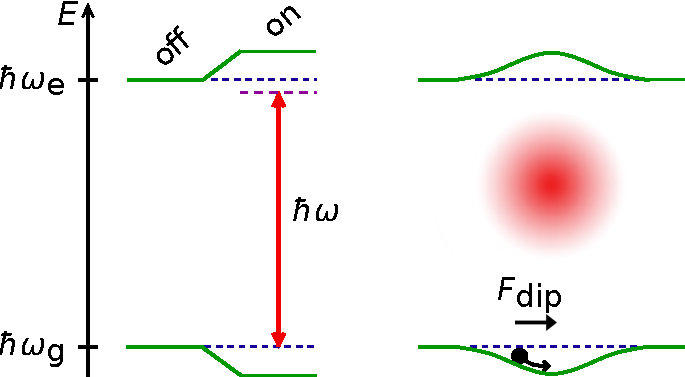
\includegraphics[height=3.8cm]{figures/LightShift.pdf}
	\caption{Light shift when the off-resonant laser is turned on, as well as the spatially varying light shift for a laser beam profile for $\delta<0$. Figure not to scale.}
	\label{fig:DipoleForce}
\end{figure}

\begin{equation}\label{eq:Stark}
	\Delta E_{e,g} \sim \pm \frac{\hbar \Omega^2}{4 \delta}.
\end{equation}

The light shift is proportional to the light intensity over the detuning: $\Omega^2 / \delta \propto I / \delta$, which we already found for the classical treatment in \cref{eq:DipoleClassicalResult}. This behavior of \cref{eq:Stark} is shown in \cref{fig:DipoleForce}. Because the field is off-resonant, atoms only occupy the ground state. For $\delta <0$ ('red detuned'), the ground state light state is negative. To calculate the new eigenstates, we repeat the treatment for a quantized light field. This is known as the dressed atom picture.

\subsection{Dressed Atom Picture}\label{sec:DressedApproach}

To calculate the new shifted eigenstates, the full Hamiltonian has to be considered, included a quantized light field with Hamiltonian $\mathcal{H}_L$ \cite{Dalibard1985}

\begin{equation}
	\mathcal{H} = \mathcal{H}_A + \mathcal{H}_L + \mathcal{H}_I(t)
\end{equation}

where the light field has eigenenergies separated by the photon energy and eigenstates of $n$ photons: $\ket{n}$ \cite{Vredenbregt2020}

\begin{equation}\label{eq:RadiationModes}
	\mathcal{H}_L = \sum_n \hbar \omega \left(n+\frac{1}{2}\right) \ket{n}\bra{n}
\end{equation}

The eigenmodes of the light field can only couple to one energy pair of the $\mathcal{H}_A + \mathcal{H}_I$ part, such that the Hamiltonian can be written down as a direct product of 2 x 2-matrix Hamiltonians \cite{Vredenbregt2020,Hussin2005} $\mathcal{H}_n$:

\begin{equation}\label{eq:CunningsHamiltonian}
    \mathcal{H}_n = \hbar 
    \begin{pmatrix}
        (n + 1)\omega -\omega_0 / 2                     & -\frac{1}{2}\sqrt{\Omega^2+\delta^2(n+1)} \\
        -\frac{1}{2}\sqrt{\Omega^2 + \delta^2(n+1)}  & n\omega + \omega_0/2
    \end{pmatrix}
\end{equation}

This is known as the Jaynes-Cummings Hamiltonian, which is one of the few problems in quantum optics analytically solvable. It has eigenvalues \cite{Hussin2005}

\begin{equation}\label{eq:CunningsEigenvalues}
    E_{\pm} = \hbar\omega\left(n+\frac{1}{2}\right) \pm \frac{\hbar}{2} \sqrt{\delta^2 + \Omega^2(n+1)}.
\end{equation}

Note the similarity to \cref{eq:SemiClassicalEigenvalues}. From \cref{eq:CunningsEigenvalues} the new eigenstates can be found to be \cite{Hussin2005}

\begin{subequations}\label{eq:CummingsEigenstates}
    \begin{align}
        \ket{+,n} &= \cos{({\theta_n}/2)} \ket{n+1,g} -\sin{(\theta_n/2)} \ket{n,e}, \\
        \ket{-,n} &= \sin{(\theta_n/2)}\ket{n+1,g} + \cos{(\theta_n/2)} \ket{n,e}.
    \end{align}
\end{subequations}

Which are sketched in \cref{fig:DipoleForce} as well. In \cref{eq:CummingsEigenstates} the mixing angle $\theta_n$ for $n$ photons in the system is

\begin{equation}
    \theta_n = \arctan{\left(
        \frac{\Omega\sqrt{n+1}}{\delta}
    \right)}
\end{equation}

Here, \cref{eq:CummingsEigenstates} are known as the \emph{dressed} states. The \emph{bare} atomic states in \cref{fig:2LevelAtom} are shifted by the light shift because the light field energy is admixed with the atomic eigenstates, leading to the new mixed (dressed) eigenstates of \cref{eq:CummingsEigenstates}. The bevavior pictured in \cref{fig:DipoleForce} still applies, but if the eigenenergies of the light field are included, the splitted energies of \cref{fig:DipoleForce} are situated along an infinite ladder of photon energies. This is presented in \cref{fig:DressedStatePicture}. The light space eigenenergies \cref{eq:RadiationModes}, spaced by $\hbar \omega$ is superimposed on the light shift eigenenergies. 

\begin{figure}
    \centering
    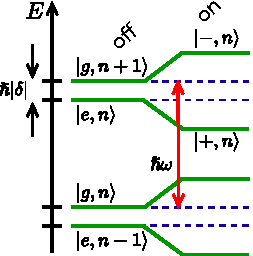
\includegraphics[width=0.31\linewidth]{figures/DressedStates.pdf}
    \caption{Dressed States. The same shift as shown in \cref{fig:DipoleForce} is shown, superimposed on the  eigenenergies spaced by $\hbar \omega$. Figue not to scale. }
    \label{fig:DressedStatePicture}
\end{figure}


\section{Strontium}\label{sec:Sr}

Historically, people started laser cooling experimentation on group 1 or alkali atoms (Na, Rb, Cs). Because they only have one valence electron, the level structure is relatively straightforward. Also, diode lasers are available for their transition frequencies. In this work, trapping of \textsuperscript{85}Rb (an alkali) is described in \cref{ch:implementation}.

However, also group 2 atoms, also called alkali-earth (and similar atoms like Yb) are possible candidates. Because of their two valence electrons, the level structure is much more complicated, making laser cooling harder, but possibly also opening up new possibilities. The element we wish to use for our new machine in Eindhoven is Sr. For more extensive coverage of Sr, the reader is referred to \cite{Stellmer2013}. Three of them are bosonic, with ${}^{88}$Sr being the most abundant at $\sim82.6\%$. There is one stable fermionic isotope: ${}^{87}$Sr has a nuclear spin of $I=9/2$ and an abundance of $\sim7.0\%$ \cite{Coursey1999}. Initially, we plan to run the machine in Eindhoven on \textsuperscript{88}Sr. Because of the lack of hyperfine structure, this isotype is a bit easier to work with, but in principle, one can use all isotopes in the same machine as the energy splitting between the isotopes is in the MHz regime, easily covered by AODs and EOMs \cite{Stellmer2013}.

\subsection{Relevant Transitions}

A simplified version of the level diagram of \textsuperscript{88}Sr is shown in \cref{fig:SrLevel}. The notation is $(n_1l_1 n_2l_2)^{2S+1}L_J$ where $n_{1,2}$ is the principal and $l_{1,2} = s, p, d, \ldots$ the azimuthal quantum number. Furthermore $S$, $L$ and $J$ are the total spin, orbital angular momentum, and total angular momentum respectively \cite{Cowan1981}.  This level scheme shows 6 out of 7 lasers to be used in this experiment. 

\begin{itemize}
	\item 461 nm. Broad transition, meaning a strong scattering force (\cref{eq:ScatteringFrequency} and high aborption-emmision cycling frequency. This is useful to slow down the hot atomic beam coming from the oven, as well as catching the atoms in a so-called blue \ac{MOT} with 'hot' temperatures of $\sim$ 1 mK.)
	
	\item 689 nm. Being much narrower than the blue transition, its Doppler temperature \cref{eq:DopplerTemperature} is much lower at $179$ nK, although in practice cooling is limited by the recoil limit to some $\sim 1$ $\mu$K \cite{Stellmer2013,Boyd2007}.
	
	\item 698 nm. The ultra-narrow clock transition ($\gamma = 1$ mHz). Used in atomic clocks because of its spectroscopic accuracy \cite{Bloom2014}. It will turn out that this feature can be put to good use in quantum computers as well, and we will use it to coherently 'drive' the qubits between the qubit basis states using this clock transition. More about this in \cref{sec:QubitScheme}
	
	\item 679, 688, and 707 nm. All repump lasers. 707 and 688 are used to cycle back atoms from ending up in ${}^3P_2$ from the decay channel shown by the grey dotted line in \cref{fig:SrLevel}. 679 is used to prevent repump leaks to ${}^3P_0$ \cite{Stellmer2013,Xu2003}.
\end{itemize}

There will also be a 813 nm laser used for the dipole trapping. This is also the most powerful laser, as it determines the limit of optical dipole traps (optical tweezers) one can make. More about this transition in \cref{sec:Magic}.

\begin{figure}
	\centering
	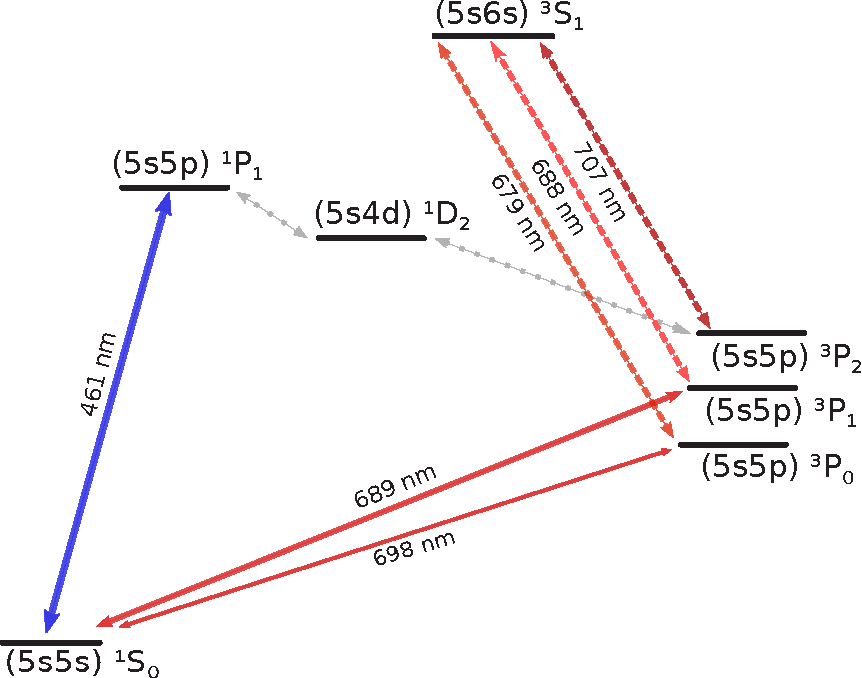
\includegraphics[width=0.51\linewidth]{figures/SrLevel.pdf}
	\caption{Simplified level scheme for \textsuperscript{88}Sr. Shown: blue transition for initial slowing and cooling. Narrower 689 nm transition of the red \ac{MOT}, and the \textsuperscript{1}S\textsubscript{0} - \textsuperscript{3}P\textsubscript{0} clock transition, which we will be used to drive the qubits. To increase density and trap lifetime 3 repump lasers are used. Not shown: 813 nm dipole trapping laser because it is driven far-off-resonant. Energies not to scale. Figure made by Ivo Knottnerus.}
	\label{fig:SrLevel}
\end{figure}

\subsection{Laser Cooling and Trapping of Sr}

Because the melting temperature of Sr is $777$ ${}^{\circ}$C, to get any relevant vapor pressure, the Sr is heated in an oven after which it sublimates. To obtain a small atomic beam divergence, the atoms are directed through a bundle of high aspect ratio capillary tubes \cite{Stellmer2013}. 

Because of the oven, the atoms are moving way too fast to be efficiently captured by the MOT. Therefore, they are slowed by a Zeeman slower. This machine uses a similar design used in the optical molasses technique, only the slowing beam is only opposing the atomic beam and not traveling along with it. A spatially varying magnetic field ensures a wide range of velocities is at some point resonant with the laser according to \cref{eq:DetuningFull}. 

Depending on the length of the Zeeman slower, only a fraction of the atoms will be slowed. To separate the hot from the cool atoms (the former are unwanted in a vacuum chamber) a deflection stage is used. The blue transition of Sr is used for this stage because of the strong scattering force. The Zeeman slowing and deflection stage is explained more elaborately in the thesis of Rik van Herk \cite{Herk2022}.

After the deflection stage, the atomic beam enters a glass cell. The advantage of using a glass cell is that it allows for the maximum amount of optical axis. To allow for longer trap survival times, the glass cell has \ac{UHV} which is separated from the stages preceding it by a differential pumping stage. 

\begin{figure}
	\centering
	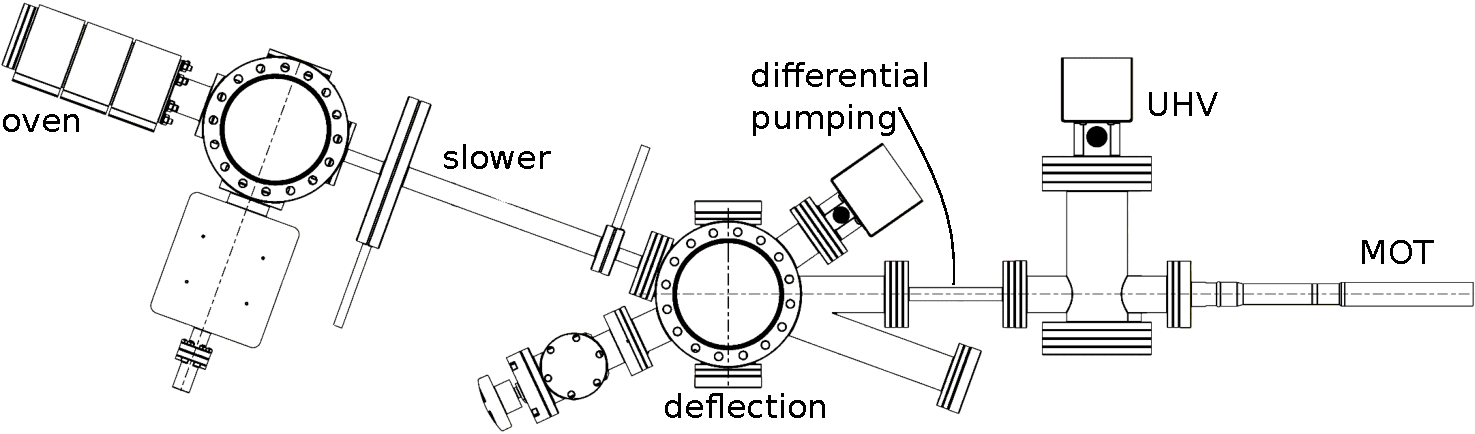
\includegraphics[width=0.8\linewidth]{figures/SrLoading.pdf}
	\caption{Sketch of the vacuum atom source design and vacuum chambers. Starting from the oven, the atomic beam traverses a Zeeman slower, deflection stage, and differential pumping stage before ending in the glass cell (MOT, right). The author did not contribute to this design. Figure by Patrick de Laat.}
	\label{fig:SrLoading}
\end{figure}

\subsection{Strontium as a Qubit}\label{sec:QubitScheme}

One of the main reasons we want to use strontium atoms for the quantum processing unit is the ${}^3P_0$ state and its very long lifetime. The clock transition is forbidden according to selection rules and only opens up after applying a magnetic field for the \textsuperscript{88}Sr isotope. Therefore,  ${}^3P_0$ is called meta-stable and can be considered a ground state on the time scale of the operation of a quantum processing unit. ${}^1S_0$ is the other clock state. Therefore, we effectily have two ground states and we can denote our qubit states as $\ket{g_1}$ and $\ket{g_2}$ (the clock states) as

\begin{equation}\label{eq:QubitManifold}
	\big\{\ket{0},\ket{1}\big\} = 
	\left\{
		\ket{{}^1S_0}, \ket{{}^3P_0} 
	\right\} = 
	\left\{ 
	    \ket{g_1}, \ket{g_2}
	\right\}.
\end{equation}

So we have two long-lifetime states connected by an extremely narrow linewidth coupling between them, that can be used to drive the qubits on the Bloch spheres. To entangle the qubits, Rydberg dressing can be used \cite{Wu2021} where a small part of a Rydberg state $\ket{r}$ is admixed in the higher energy ground state:

\begin{equation}\label{eq:RydbergDressing}
	\ket{\psi} \sim \ket{g_2} + \epsilon \ket{r}
\end{equation}

The amount of dressing is tuned by the (small) dressing parameter $\epsilon \propto \Omega / 2\delta$ where $\Omega$ is the Rabi frequency of the laser and $\delta$ the usual detuning. A Rydberg state is an electronic state with a very high principal quantum number $n$. Rydberg atoms are physically larger, as the electron orbit radius scales $\propto n^2$ \cite{Gallagher1994}. As a result of these exaggerated electron orbit sizes, neighboring atoms can 'feel' each other. For example, the van der Waals interaction coefficient scales as $\propto n^{11}$ \cite{Gallagher1994}. 

Other qubit implementations than the one above are possible as well. For example, \cite{Barnes2021} uses the fermionic ${}^{87}$Sr and maps the qubit states onto the nuclear spin states $\ket{{}^1S_0, F=9/2, m_F = -9/2}$ and $\ket{{}^1S_0, F=9/2, m_F = -7/2}$.

\subsubsection*{Magic Trapping of Strontium}\label{sec:Magic}

\begin{figure}
    \centering
    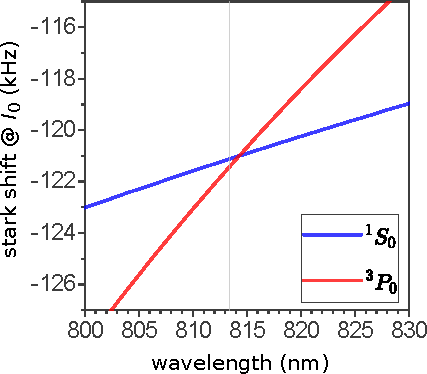
\includegraphics[width=0.38\linewidth]{figures/Magic.pdf}
    \caption{Atomic polarizabilities of ${}^1S_0$ and ${}^3P_0$ showing a magic crossing around 813 nm. Grey line: experimental result. Figure adapted from \cite{Boyd2007}.} 
    \label{fig:BoydMagic}
\end{figure}

To use the states in \cref{eq:QubitManifold} in a quantum processing unit, they should both be trapped. Because the trapping potential is wavelength dependent, in general, the trapping potential will not be the same for both qubit states when using the same trapping wavelength (\cref{eq:DipoleForce}: $U_{\text{dip}} \propto - \operatorname{Re}\{\alpha(\omega)\} I(\mathbf{r})$, meaning that the transition frequency between the qubit states would change as a function of the position within the potential which is unfavorable. Instead, \cite{Katori2003} proposed to use a wavelength where the polarizability $\alpha(\omega)$ or $\alpha(\lambdaup)$ is identical for both clock states as measured by \cite{Takamoto2005,Jun2008}.

Calculating this \textit{magic} crossing point of \cref{eq:MagicCrossing} is outside the scope of this thesis, but we will show the final result as found by \cite{Boyd2007} in \cref{fig:BoydMagic}. The reader is referred to \cite{Madjarov2020,Boyd2007} for more information. Plotting the polarizability for both clock states as a function of wavelength and one findes a magic crossing point around 813 nm. By trapping both qubit states in the same potential, one can coherently drive the qubits to any point on the Bloch spheres. 

Both qubit states coupled far-off-resonantly to a different excited states using this same magic potential. The excited states used can be found in \cref{fig:SrLevel}. That figure is one again plotted in \cref{fig:2LevelTweezer}, where the two different dipole trap schemes are highlighted.

\begin{equation}\label{eq:MagicCrossing}
    \operatorname{Re}\left\{\alpha(\lambdaup-\lambdaup_{\ket{g_1})})\right\} = 
    \operatorname{Re}\left\{\alpha(\lambdaup-\lambdaup_{\ket{g_2})})\right\}
\end{equation}

\begin{figure}
    \centering
    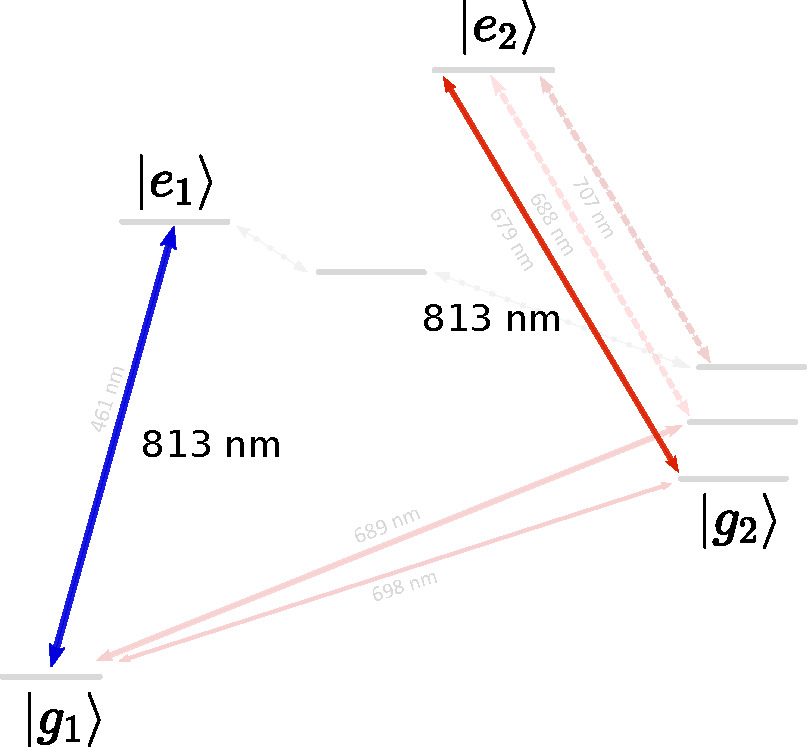
\includegraphics[width=.38\linewidth]{figures/2groundTweezer.pdf}
    \caption{Both clock states, here denoted $\ket{g_1}, \ket{g_2}$ are coupled to a different excited state: $\ket{e_1}, \ket{e_2}$ using the same trapping laser at 813 nm.}
    \label{fig:2LevelTweezer}
\end{figure}



	

